\documentclass[a4paper, twoside]{article}
\usepackage[utf8]{inputenc} % Especifica la codificación de caracteres de los documentos.
\usepackage[spanish]{babel} % Indica que el documento se escribirá en español.
\usepackage[top=3cm, bottom=2.5cm, inner=1.5cm, outer=2.5cm]{geometry} % Márgenes personalizados
\usepackage{subfiles} % Paquete para incluir el preambulo en los sub archivos.
\usepackage{afterpage} % Permite añadir páginas despues de una página dada.
\usepackage{hyperref} % Permite incluir enlaces en los archivos.
\usepackage{lastpage} % Paquete para poder contabilizar el total de páginas del documento.
\usepackage{fancyhdr} % Permite personalizar los header y footer del documento.
\usepackage{graphicx} % Permite incluir gráficos
\usepackage[hang, bf]{caption} % Personaliza los subtítulos de las figuras y tablas
\usepackage{float} % Permite posicionar mejor las figuras y tablas
\usepackage{listings} % Permite insertar código fuente
\usepackage{xcolor} % Permite utilizar más colores.

\definecolor{darkblue}{rgb}{0,0,0.4}
\definecolor{darkgreen}{rgb}{0,0.4,0}

% Defino la ruta de los paquetes personalizados para el apunte
\newcommand{\rutapaquetes}{./paquetes-apunte}

\usepackage[mostrarlicencia]{\rutapaquetes/caratula} % Caratula personalizada (cargada desde caratula.sty)
\usepackage[mostrarrevisores]{\rutapaquetes/colaboradores} % Seccion de colaboradores (cargada y creada con colaboradores.sty)
\usepackage{\rutapaquetes/historial} % Seccion de historial de cambios (cargada y creada con historial.sty)

% Define los estilos de los enlaces interpretados por el paquete hyperref
\hypersetup{
	colorlinks=true,   % false: boxed links; true: colored links
	linkcolor=black,   % color of internal links (change box color with linkbordercolor)
	citecolor=green,   % color of links to bibliography
	filecolor=magenta, % color of file links
	urlcolor=blue     % color of external links
}

\newcommand{\imgdir}{../resources/images} % Ruta de las imágenes

% Define los directorios de las imágenes y gráficos
\graphicspath{ {\imgdir/} {\rutapaquetes/} }

\newcommand{\nombremateria}{Sistemas Operativos (75.08 - 95.03)} % Defino el comando "\nombremateria" para no harcodear el nombre en varios lugares.

% Define el pagestyle personalizado
\pagestyle{fancy}
\fancyhf{}
\renewcommand{\sectionmark}[1]{\markboth{}{\thesection\ \ #1}}
% Define header para pagina par
\fancyhead[ER]{\rightmark}
% Define header para pagina impar
\fancyhead[OL]{\rightmark}
% Define footer para pagina par
\fancyfoot[EL]{\nombremateria} % Nombre del apunte a la izquierda
\fancyfoot[ER]{Página \thepage\ de \pageref{LastPage}} % Numero de pagina a la derecha
% Define footer para pagina impar
\fancyfoot[OL]{Página \thepage\ de \pageref{LastPage}} % Numero de pagina a la izquierda
\fancyfoot[OR]{\nombremateria} % Nombre del apunte a la derecha

\renewcommand{\footrulewidth}{0.4pt} % Agrego linea que separa el footer

% Elijo formato de bloques de código fuente
\lstset{ 
	backgroundcolor=\color{white},
	basicstyle=\ttfamily\footnotesize,
	breaklines=true,
	commentstyle=\color{darkgreen},
	extendedchars=true,
	frame=single,
	language=C++,
	literate={á}{{\'a}}1 {é}{{\'e}}1 {í}{{\'i}}1 {ó}{{\'o}}1 {ú}{{\'u}}1 {ñ}{{\~n}}1, % Escapeo caracteres especiales
	keywordstyle=\color{darkblue},
	numbers=left,
	numberstyle=\tiny\color{gray},
	tabsize=4,
	showspaces=false,
	showstringspaces=false,
	stringstyle=\color{red}
}

% Configura la caratula
\materia{\nombremateria}
\tipoapunte{Resumen teórico}
%\tema{Tema de la Materia}
%\subtema{Subtema}

\begin{document}
% Página en blanco agregada después de la carátula
%\afterpage{
%	\null
%	\thispagestyle{empty}%
%	\addtocounter{page}{-1}%
%	\newpage}
\maketitle % Genera la carátula

\tableofcontents % Genera el índice

\subfile{\rutapaquetes/acerca-del-proyecto.tex} % Incluye información acerca del proyecto FIUBA Apuntes

% Insertar aquí el contenido del apunte. A continuacion hay secciones a modo de ejemplo.

\section{Introducción}
\subsection{¿Qué es un sistema operativo?}
\begin{itemize}
	\item Un programa que hace de intermediario entre el usuario de la computadora y su hardware (Oculta los detalles finos de la arquitectura).
	\item Un programa que administra los recursos de un sistema de computación: permite administrar el tiempo de procesador y el espacio (memoria, disco, etc).
\end{itemize}

\subsection{Arquitecturas}
\subsubsection{Mainframe}
Computadora central. Gran capacidad de I/O, server para e-commerce a gran escala.\\

\textbf{Seguridad y disponibilidad:} 
\begin{itemize}
	\item Transaction processing: es procesamiento de información distribuido en operaciones individuales e indivisibles, llamadas \emph{transacciones}. Cada transacción debe ser exitosa o fallar como unidad entera, no puede haber transacciones parcialmente completas.
	\item Batch processing: Es la ejecución de una serie de programas ("tareas") en una computadora sin intervención del usuario.
\end{itemize}

\subsubsection{Servidores}
Destinados a ofrecer servicios a través de una red.

\subsubsection{Supercomputadoras}
Computacion de alto rendimiento. Se usan para hacer simulaciones.\\

\textbf{Limites:}
\begin{itemize}
	\item Concurrencia: los procesos no son 100\% independientes
	\item Costo
	\item Programación del software
\end{itemize}

\subsubsection{Server operating system}
Interfaz solo línea de comando o EFI (estándar de firmware).

\subsubsection{Computadora personal}
No requiere conocimientos especiales.

\subsubsection{Tablets, PDA}

\subsubsection{Consolas}

\subsubsection{Sistemas operativos embebidos}
Dispositivos que no aceptan instalación de nuevo software por el usuario.

No deberían tener bugs.

Se usan en tvs, autos, etc.

\subsubsection{Cluster}
Un grupo de computadoras interconectadas por una red local de alta velocidad.

Se comportan como si fuese una única computadora.

Si es de alta disponibilidad tiene nodos redundantes en caso de falla. Retoma en otro equipo en el estado en el que estaba. 

Balance de carga, con dispositivo físico o de software.

\subsubsection{Grid}
Cluster virtual con recursos distribuidos.

\textbf{Ejemplo:} BOINC, SETI.

\textbf{Problemas:} concurrencia (que se choquen tareas), que queden tareas sin cubrir.

\subsubsection{Cloud computing}
Se provee por internet. Dinamicamente escalable.

Atrás de la nube puede haber cluster, grid, etc (al cliente no le importa).

\textbf{Servicios posibles de cloud computing:}
\begin{itemize}
	\item Cloud Storage: Dropbox.
	\item Infraestructura (infraestructura as a service (IaaS)):Tipicamente plataformas virtualizadas. Ejemplo: Amazon EC2
	\item Plataforma (PaaS): Provee la plataforma y un ambiente de desarrollo y soporte. Ejemplo: Google Code.
	\item Software (SaaS): Software on demand provisto por terceros. Ejemplo: Amazon Services, Paypal. 
\end{itemize}

\subsubsection{Tiempo real}
Distinto de online o de rápido.

Tiempo de respuesta máximo y predecible. 

\subsubsection{Multiprocesador}
Más de un procesador en el mismo chip o board.

Soportado en todos los sistemas operativos de escritorio.

La paralelizacion esta limitada por la ley de Amdahl: El \emph{speedup} de un programa que utiliza varios procesadores en paralelo está limitado por el tiempo tomado por la fracción secuencial del programa.

\newpage
\section{Mecanismos básicos}
Sistema operativo es software que extiende un poco la capa de hardware.

El hardware es lo que le provee recursos al sistema operativo: CPU, memoria, dispositivos I/O. Cada nivel interpreta al nivel superior.

El estado de una maquina virtual sólo está definido entre instrucción e instrucción.

Una instrucción en una capa equivale a muchas instrucciones de la capa inferior.

\subsection{Modos de CPU}
Son distintos niveles de permisos o privilegios.

Se suele trabajar con dos modos: \textbf{Modo Supervisor} (puede hacer todo) y \textbf{Modo Usuario} (tiene restricciones).

Se pasa de modo usuario a modo supervisor por medio de una interrupción. 

El retorno a modo usuario está a cargo del programa. Motivo para querer pasar de modo supervisor a modo usuario: Control de riesgo de código desconocido (ejemplo: escribir en las direcciones de memoria del SO).\\

Algunas arquitecturas incluyen más modos:
\begin{itemize}
	\item X86 Modo real, protegido y virtual.
	\item Modo hypervisor
\end{itemize}

Un sistema operativo puede tener partes corriendo en cada uno de los modos.

Un programa de usuario sólo corre en modo usuario. El único programa que debiera ser capaz de pasar a modo supervisor es el sistema operativo.

\subsection{Interrupciones}
Una interrupción es una suspensión temporal de la ejecución de un proceso, para pasar a ejecutar una subrutina de servicio de interrupción, la cual, por lo general, no forma parte del programa, sino que pertenece al sistema operativo o al BIOS. Una vez finalizada dicha subrutina, se reanuda la ejecución del programa.\\

Hay dos tipos de interrupciones:
\begin{itemize}
	\item Sincronica o software trap: Una instrucción del programa.
	\item Asincrónica: I/O, timer, external.
\end{itemize}

\subsubsection{Atención de interrupciones}
\begin{enumerate}
	\item \textbf{Primer nivel de atención:} Salvar el contexto (registros, código de condición, dirección de retorno). El objetivo es poder proseguir el proceso (después de atendida la interrupción) desde el estado en el que estaba. Que un proceso sufra o no una interrupción no cambia su resultado, solamente el tiempo que le insume.
	
	\item \textbf{Segundo nivel de atención:} Se decide si se atiende en el momento la interrupción o se deja para después. Si vienen 2 interrupciones al mismo tiempo puede llegar a perderse una. Por eso los que envían la interrupción deben estar preparados para repetirla.
\end{enumerate}

\subsection{Modos del sistema operativo}
\subsubsection{Modo Kernel}
Ejecutando un servicio propio del sistema operativo.

En computación, el \emph{kernel} es un programa que maneja las solicitudes de entrada y salida que realiza el software, traduciendolas en instrucciones de procesamiento de datos para la CPU y otros componenentes electrónicos de una computadora. El kernel es una parte fundamental en un sistema operativo moderno de PC.

Debido a su naturaleza crítica, el código kernel generalmente se encuentra cargado en un area protegida de la memoria, previniendo que sea sobreescrito por otra parte no tan usada del sistema operativo o por aplicaciones. El kernel realiza sus tareas, como la ejecución de procesos y manejo de interrupciones, en area del kernel, mientras que todo lo que un usuario normalmente haría, como escribir texto en un editor o correr aplicaciones con interfaz gráfica, se realiza en el espacio del usuario. Esta separación se realiza con el fin de prevenir datos del usuario y del kernel interferir uno con el otro, disminuyendo performance o causando el sistema operativo inestable (o incluso colgandolo)

Cuando un programa (o como se lo conoce en este contexto \emph{proceso}) realiza solicitudes al kernel, esta solicitud se llama "llamada al sistema" o \emph{system call}

\subsubsection{Modo usuario}
Ejecutando un programa de usuario.

The term userland (or user space) refers to all code which runs outside the operating system's kernel. Userland usually refers to the various programs and libraries that the operating system uses to interact with the kernel: software that performs input/output, manipulates file system objects, application software etc.

\subsection{System Calls}
Si un proceso esta corriendo un programa en modo usuario y necesita un servicio del sistema, como leer data de un archivo, tiene que ejecutar un software trap para transferirle el control al sistema operativo. El sistema operativo se fija lo que necesita el proceso que lo  llamo inspeccionando los parámetros. Hace lo que tenga que hacer y devuelve el control a la instrucción que sigue al system call.\\

Ejemplos
\begin{itemize}
	\item Leer de un dispositivo solo puede hacer el SO (leer de memoria, CD, USB, etc).
	\item Manejo de procesos
	\item Manejo de archivos
	\item Etc
\end{itemize}

\subsection{Library Calls}
Son llamados a procedimientos de bibliotecas provistas por el lenguaje en el que se está programando.\\

\begin{figure}[H]
	\centering
	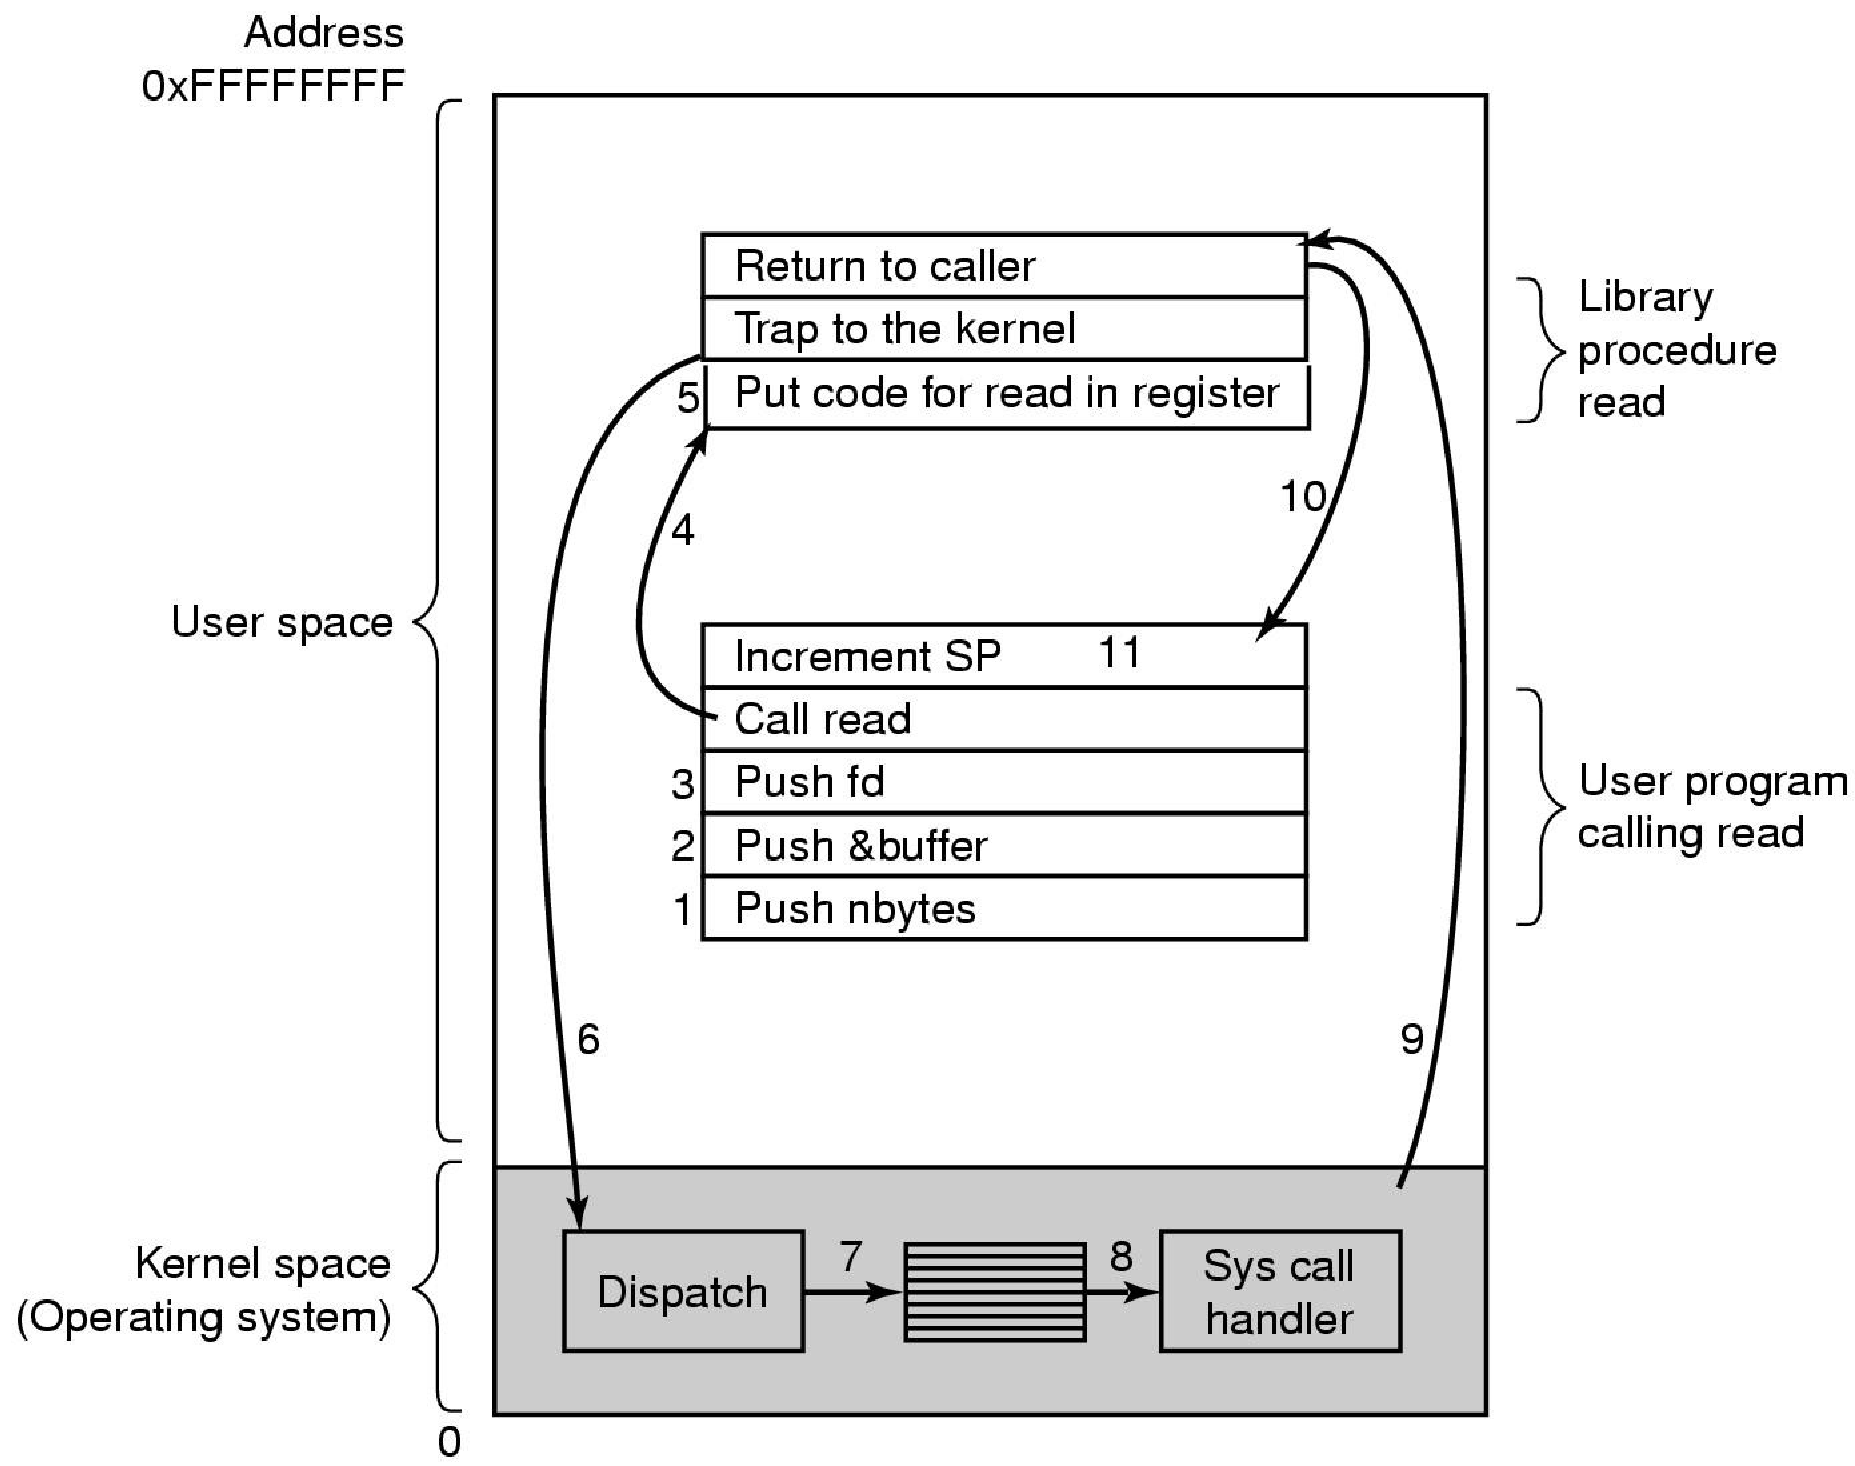
\includegraphics[width=0.7\textwidth]{library_call}
	\caption{Llamado a procedimientos de bibliotecas}
	\label{fig:library_call}
\end{figure}

Referencias de la Figura \ref{fig:library_call}:
\begin{itemize}
	\item 1, 2, 3 y 4 corresponden a un llamado convencional a un procedimiento.
	\item Antes de hacer 5, el sistema operativo habilita el acceso a la memoria del sistema operativo (pasa a modo kernel).
	\item 6 implica una software trap, el procesador pasa a modo protegido.
	\item 7 y 8 se ejecutan en modo protegido del procesador.
	\item En 9 se vuelve a modo usuario del procesador, pero con el sistema operativo en modo kernel.
	\item El paso 10 reestablece la protección de memoria del sistema operativo (sale de modo kernel).
\end{itemize}

\newpage
\section{Procesos}
\subsection{Modelo de procesos}
El sistema operativo debe organizar el software que corre en unidades secuenciales, a esta organización se le llama proceso.\\

Un proceso es:
\begin{itemize}
	\item La imagen de un programa en ejecución (una copia del programa).
	\item Con las estructuras del sistema operativo para administrarlo.
	\item Varios procesos pueden estar asociados a un mismo programa; por ejemplo, iniciar varias instancias de un mismo programa generalmente significa que más de un proceso está siendo ejecutado.
\end{itemize}

Un proceso tiene:
\begin{itemize}
	\item La imagen del programa (una copia de su código ejecutable y de su área de datos).
	\item La información acerca de sus estado de ejecución:
	\begin{itemize}
		\item Los valores del program counter, registros y variables.
		\item Información necesaria para su administración por parte del Sistema Operativo (id, prioridad, ...).
	\end{itemize}
	\item Memoria (generalmente una región de memoria virtual); que incluye el código ejecutable, datos específicos del proceso (entrada y salida), un stack de llamadas (para mantener registro de las subrutinas activas y otros eventos), y un heap para mantener datos intermedios generados durante el tiempo de ejecución.
	\item Descriptores de recursos del sistema operativos, reservados por el proceso, como pueden ser los \emph{file descriptors} (Unix), o \emph{handles} (Windows), y fuentes y sumideros de datos.
	\item Atributos de seguridad, como el propietario del proceso y los permisos (operaciones permmitidas) del mismo.
\end{itemize}

Esta información la guarda el sistema operativo en estructuras de datos llamadas \emph{Process Control Blocks}.\\

Cualquier subgrupo de recursos, menos, generalmente, el estado del procesador, puede estar asociado con cada uno de los threads del proceso (en sistemas operativos que soportan threads) o en los procesos "hijos".

El sistema operativo mantiene sus procesos separados y reserva los recursos que necesitan, de manera que sean menos propensos a interferir entre ellos y causen fallas del sistema (como deadlocks o thrashing). El sistema operativo también provees mecanismos para la comunicación entre procesos, permitiendoles interactuar de manera segura y predecible.

\subsection{Multiprogramación}
En computación, \emph{multitasking} es un metodo donde multiples tareas (procesos) son ejecutadas durante el mismo periodo de tiempo. Se ejecutan \emph{concurrentes} (en periodos de tiempo solapados, una tarea puede iniciar antes que otras hayan terminado) en vez de \emph{secuenciales} (una tarea comienza luego de que la anterior haya terminado). Las tareas concurrentes comparten recursos de procesamiento, como la CPU y memoria principal.\\

Multitasking no necesariamente significa que varias tareas se ejecutan en el mismo preciso momento. En otras palabras, multitasking NO implica paralelismo, pero si significa que más de una tarea puede estar en medio de su ejecución al mismo tiempo, y que mas d euna tarea está avanzando dentro de un periodo de tiempo determinado.

En caso de una computadora con un solo CPU, solo una tarea se dice estar corriendo en determinado tiempo, lo que significa que ese CPU está activamente ejecutando instrucciones para esa tarea.\\
Multitasking resuelve este problema organizando qué tarea se ejecutará en cada tiempo determinado, y cuándo una tarea en espera obtiene un turno. El acto de reasignar un CPU de una tarea a otra se llama \emph{context switch}, o cambio de contexto. Cuando estos cambios de contexto ocurren lo suficientemente seguidos, se logra una ilusión de paralelismo.

Incluso en computadoras con más de un CPU (máquinas \emph{multiprocesadores}) o más de un nucleo en determinado CPU (máquinas \emph{multinúcleo}), donde más de una tarea puede ser ejecutada en un determinado instante (una por núcleo), multitasking permite correr muchas más tareas que la cantidad de CPUs presentes.

Cuando hay más de un procesador se conoce como Multiprocesamiento.

Se ejecuta un proceso. Cuando se “bloquea” por I/O, se aprovecha el tiempo para ejecutar otro proceso.

La CPU va conmutando (switching) de un proceso a otro.

Es un multiplexado de la CPU.

\subsubsection{Implementación de la multiprogramación}
\begin{itemize}
	\item Se conoce como \emph{scheduler} al mecanismo que permite elegir varios procesos en estado \emph{Ready}, para otorgarles tiempo de CPU y que puedan realizar sus tareas. Para ello aplica un algoritmo de scheduling, que tiene en cuenta los siguientes aspectos
	\begin{itemize}
		\item Cantidad requerida de recursos.
		\item Cantidad actualmente disponible de recursos.
		\item Prioridad del trabajo o proceso.
		\item la cantidad de tiempo de espera.
	\end{itemize}
	
	\item \emph{Dispatcher} es el mecanismo que otorga tiempo de CPU al proceso seleccionado por el scheduler. Para esto, se realizan los siguientes pasos:
	\begin{itemize}
		\item Cambio de contexto (\emph{Context switching})
		\item Cambiar a modo usuario (\emph{user mode})
	\end{itemize}
	El tiempo se divide en segmentos, denominados \emph{time slices}. Cuando un \emph{time slice} se termina, le permite al scheduler actualizar el estado de cada proceso, y seleccionar el próximo a ejecutar.
\end{itemize}

Cada vez que se interrumpe un proceso también se pierde el tiempo de guardar el contexto.

\subsection{Estados de un proceso}
\begin{figure}[H]
	\centering
	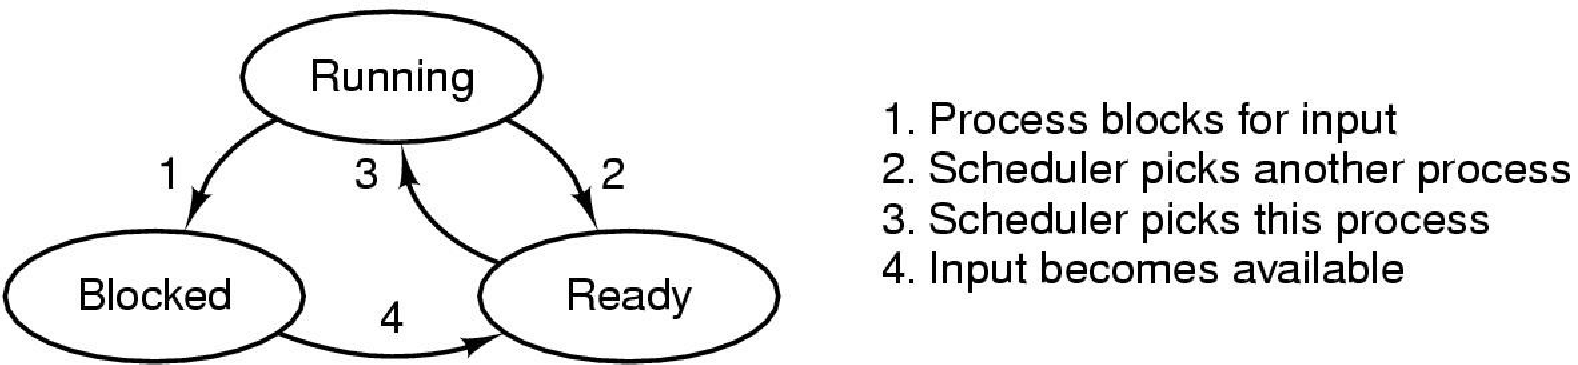
\includegraphics[width=0.7\textwidth]{process_states_simple}
	\caption{Estados de un procedimiento (simplificado)}
	\label{fig:process_states_simple}
\end{figure}

\begin{figure}[H]
	\centering
	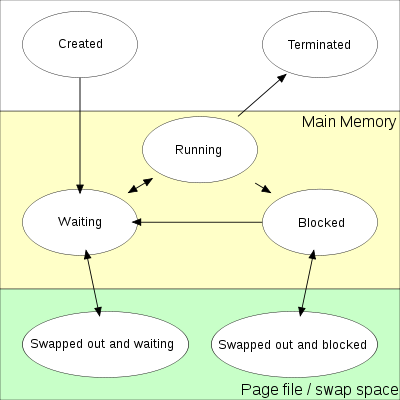
\includegraphics[width=0.5\textwidth]{process_states_full}
	\caption{Estados de un procedimiento}
	\label{fig:process_states_full}
\end{figure}

\subsubsection{Created or New}
When a process is first created, it occupies the ``created'' or ``new'' state. In this state, the process awaits admission to the ``ready'' state. This admission will be approved or delayed by a long-term, or admission, scheduler. Typically in most desktop computer systems, this admission will be approved automatically, however for real-time operating systems this admission may be delayed. In a real time system, admitting too many processes to the "ready" state may lead to oversaturation and over contention for the systems resources, leading to an inability to meet process deadlines.

\subsubsection{Ready and waiting}
A ``ready'' or ``waiting'' process has been loaded into main memory and is awaiting execution on a CPU (to be context switched onto the CPU by the dispatcher, or short-term scheduler). There may be many ``ready'' processes at any one point of the system's execution—for example, in a one-processor system, only one process can be executing at any one time, and all other ``concurrently executing'' processes will be waiting for execution.

A ready queue or run queue is used in computer scheduling. Modern computers are capable of running many different programs or processes at the same time. However, the CPU is only capable of handling one process at a time. Processes that are ready for the CPU are kept in a queue for ``ready'' processes. Other processes that are waiting for an event to occur, such as loading information from a hard drive or waiting on an internet connection, are not in the ready queue.

\subsubsection{Running}
A process moves into the running state when it is chosen for execution. The process's instructions are executed by one of the CPUs (or cores) of the system. There is at most one running process per CPU or core. A process can run in either of the two modes, namely kernel mode or user mode.

\subsubsection{Blocked (Waiting)}
A process that is blocked on some event (such as I/O operation completion or a signal). A process may be blocked due to various reasons such as when a particular process has exhausted the CPU time allocated to it or it is waiting for an event to occur.

\subsubsection{Terminated}
A process may be terminated, either from the ``running'' state by completing its execution or by explicitly being killed. In either of these cases, the process moves to the ``terminated'' state. The underlying program is no longer executing, but the process remains in the process table as a zombie process until its parent process calls the wait system call to read its exit status, at which point the process is removed from the process table, finally ending the process's lifetime. If the parent fails to call wait, this continues to consume the process table entry (concretely the process identifier or PID), and causes a resource leak.\\

A child process always first becomes a zombie before being removed from the resource table. In most cases, under normal system operation zombies are immediately waited on by their parent and then reaped by the system – processes that stay zombies for a long time are generally an error and cause a resource leak.\\

Después de terminado un proceso, el mismo queda en estado ``terminado'' hasta que el sistema operativo termina de limpiar las estructuras que usó para ejecutarlo (mientras tanto está en estado zombie).

\begin{lstlisting}
int main()
{
	pid_t child_pid;

	child_pid = fork();
	if(child_pid > 0){
		sleep(60);
	}else{
		exit(0);
	}
	return 0;
}
\end{lstlisting}

\subsection{PCB (Process Control Block)}
Es la estructura de datos con la que el sistema operativo administra los procesos.
Contiene la información acerca del proceso y su estado.
Además la información que el S.O. precisa para manejarlo como: Identificador, Estado, Recursos, Historia.
Ejemplo de datos que maneja: Registros, Program counter, Process ID, Punteros de memoria, etc.

\underline{Estados de un proceso}:
Los estados se manejan como colas.
El Dispatcher es el encargado de cambiar los PCBs entre las colas.

\subsubsection{Dispatcher (Scheduler de corto plazo)}
Decide qué proceso, entre los procesos en memoria y con estado \emph{ready}, será ejecutado (otorgado un CPU) luego de una interrupción del clock, una interrupción de entrada/salida, llamada al sistema operativo u otro tipo de señal. Por este motivo, este scheduler de corto plazo realizar tareas de planificación mucho más seguido que los schedulers de medio y largo plazo. Al menos una decisión de scheduling se realiza luego de cada \emph{time slice}, y estos son bastante cortos.

\begin{itemize}
	\item Al pasar de Running a Blocked.
	El manejador de interrupciones lo invoca para cambiar de estado al proceso:
	\begin{itemize}
		\item Salva los datos necesarios en el PCB.
		\item Cambia el PCB de cola.
	\end{itemize}
	Luego se decide a que proceso dar control (tarea del Scheduler).

	\item Al pasar de Ready a Running \\
	El Scheduler lo invoca cuando ya decidió a que proceso activar. \\
	Carga el estado de la CPU con los datos del PCB. \\
	Continúa la ejecución del proceso.
\end{itemize}

\subsubsection{Scheduler (Long term)}
Decide a cuál de los procesos en ready hay que darle el control.
In general, most processes can be described as either I/O-bound or CPU-bound. An I/O-bound process is one that spends more of its time doing I/O than it spends doing computations. A CPU-bound process, in contrast, generates I/O requests infrequently, using more of its time doing computations.
It is important that a long-term scheduler selects a good process mix of I/O-bound and CPU-bound processes. If all processes are I/O-bound, the ready queue will almost always be empty, and the short-term scheduler will have little to do. On the other hand, if all processes are CPU-bound, the I/O waiting queue will almost always be empty, devices will go unused, and again the system will be unbalanced.
he system with the best performance will thus have a combination of CPU-bound and I/O-bound processes.\\

Tiene en cuenta las características del proceso:

\begin{itemize}
	\item \textbf{Throughput} - The total number of processes that complete their execution per time unit.
	\item \textbf{Latency}, specifically:
	\begin{itemize}
		\item \textbf{Turnaround time} - total time between submission of a process and its completion.
		\item \textbf{Response time} - amount of time it takes from when a request was submitted until the first response is produced.
	\end{itemize}
	\item \textbf{Fairness} - Equal CPU time to each process (or more generally appropriate times according to each process' priority and workload).
	\item \textbf{Waiting Time} - The time the process remains in the ready queue.
\end{itemize}

\paragraph{Objetivos del Scheduler:}
\begin{itemize}
	\item Dar una participación adecuada del reparto de tiempo de CPU (Fairness).
	\item Equilibrar el uso de recursos (Load Balancing).
	\item Aplicar las políticas generales del Sistema (prioridades, afinidad, seguridad).
	\item El resto depende del tipo de Sistema.
\end{itemize}

In practice, these goals often conflict (e.g. throughput versus latency), thus a scheduler will implement a suitable compromise. Preference is given to any one of the concerns mentioned above, depending upon the user's needs and objectives.

\begin{itemize}
	\item Batch (por lotes):
	\begin{itemize}
		\item maximizar el throughput: cantidad de procesos / tiempo.
		\item Mantener la CPU ocupada.
		\item Minimizar el turnaround time.
	\end{itemize}
	\item Interactivo:
	\begin{itemize}
		\item Buen tiempo de respuesta
		\item Expectativas del usuario
	\end{itemize}
	\item Real time:
	\begin{itemize}
		\item Cumplir con los deadlines
		\item Desempeño predecible
	\end{itemize}
\end{itemize}

Las decisiones de scheduling se pueden tomar cuando un proceso:

\begin{itemize}
	\item Pasa de running a blocked/waiting. (Transicion NO apropiativa)
	\item Pasa de running a ready. (Transicion apropiativa)
	\item Pasa de blocked/waiting a ready. (apropiativa)
	\item Termina. (NO apropiativa)
\end{itemize}

\textbf{Transicion apropiativa}: es el SO el que interrumpe.

\textbf{Transcion no apropiativa}: es el propio proceso el que interrumpe.

\textbf{Starvation}: es un problema que ocurre cuando hay multitasking, donde a un proceso se le niega constantemente los recursos necesarios. De esta manera la tarea nunca puede concretarse.

\subsection{Algoritmos de scheduling}

\begin{enumerate}
	\item FIFO
	\item Shortest Job Next (SJN)
	\item Round Robin
	\item Múltiples colas con prioridad
\end{enumerate}

\subsubsection{First come-First served (FIFO)}
Simplemente encola procesos en estado \emph{ready} en el orden de llegada.\\

\textbf{Características}

\begin{itemize}
	\item Since context switches only occur upon process termination, and no reorganization of the process queue is required, scheduling overhead is minimal.
	\item Throughput can be low, since long processes can hold the CPU
	\item Turnaround time, waiting time and response time can be high for the same reasons above
	\item No prioritization occurs, thus this system has trouble meeting process deadlines.
	\item The lack of prioritization means that as long as every process eventually completes, there is no starvation. In an environment where some processes might not complete, there can be starvation.
	\item It is based on Queuing
\end{itemize}

\subsubsection{Shortest Job Next}
Selecciona para ser ejecutado el proceso en espera con el menor tiempo de ejecución.

\textbf{Pros}:
\begin{itemize}
	\item Shortest job next is advantageous because of its simplicity and because it minimizes the average amount of time each process has to wait until its execution is complete. 
\end{itemize}

\textbf{Contras}:
\begin{itemize}
	\item However, it has the potential for process starvation for processes which will require a long time to complete if short processes are continually added.
	\item Another disadvantage of using shortest job next is that the total execution time of a job must be known before execution. While it is not possible to perfectly predict execution time, several methods can be used to estimate the execution time for a job, such as a weighted average of previous execution times.
\end{itemize}

\subsubsection{Round Robin}
Time slices are assigned to each process in equal portions and in circular order, handling all processes without priority (also known as cyclic executive). 

\textbf{Pros}:
\begin{itemize}
	\item Round-robin scheduling is simple, easy to implement, and starvation-free.
	\item Good average response time, waiting time is dependent on number of processes, and not average process length.
	\item Starvation can never occur, since no priority is given. Order of time unit allocation is based upon process arrival time, similar to FCFS.
\end{itemize}

\textbf{Contras}:
\begin{itemize}
	\item Because of high waiting times, deadlines are rarely met in a pure RR system.
\end{itemize}

\subsubsection{Múltiples colas con Prioridad}
This is used for situations in which processes are easily divided into different groups. For example, a common division is made between foreground (interactive) processes and background (batch) processes. These two types of processes have different response-time requirements and so may have different scheduling needs. It is very useful for shared memory problems.
If a process uses too much CPU time, it will be moved to a lower-priority queue. This scheme leaves I/O-bound and interactive processes in the higher priority queues. In addition, a process that waits too long in a lower-priority queue may be moved to a higher priority queue. This form of aging also helps to prevent starvation of certain lower priority processes.

\subsection{Creacion/Terminacion de procesos}
\subsubsection{Creación de Procesos}
\begin{itemize}
	\item Al iniciar el sistema (Booting)
	\item Por pedido del usuario (Uso de una System Call).
\end{itemize}

\subsubsection{Terminación de procesos}
\begin{itemize}
	\item Salida normal (voluntaria).
	\item Salida por error (voluntaria).
	\item Error “fatal” (involuntaria).
	\item “Muerte” por otro proceso.
\end{itemize}

\subsection{Booting}
A boot loader is a computer program that loads an operating system or some other system software for the computer after completion of the power-on self-tests; it is the loader for the operating system itself, which has its own loader for loading ordinary user programs and libraries. Within the hard reboot process, it runs after completion of the self-tests, then loads and runs the software. A boot loader is loaded into main memory from persistent memory, such as a hard disk drive or, in some older computers, from a medium such as punched cards, punched tape, or magnetic tape. The boot loader then loads and executes the processes that finalize the boot.

\begin{itemize}
	\item Cargar en memoria un software que pueda lanzar un Sistema Operativo.
	\begin{itemize}
		\item Switches en el panel.
		\item Flash boot loader.
		\item MBR (Master Boot Record) program.
		\item EFI (Extended Firmware Interface).
	\end{itemize}
	\item Termina cargando el first stage boot loader.
\end{itemize}

\subsection{EFI (Extensible Firmware Interface)}
Interfaz Extensible del Firmware, Extensible Firmware Interface (EFI), es una especificación desarrollada por Intel dirigida a reemplazar la antigua interfaz del estándar IBM PC ROM BIOS, e interactúa como puente entre el sistema operativo y el firmware base.

\begin{itemize}
	\item Boot Services:
	\begin{itemize}
		\item Soporte de consola.
		\item Soporte gráfico.
	\end{itemize}
	\item Runtime Services:
	\begin{itemize}
		\item Device Drivers
		\item Fecha y Hora
	\end{itemize}
	\item Carga de código desde Internet
\end{itemize}

Las especificaciones de la EFI permiten ofrecer un controlador de dispositivo independiente del procesador denominado EFI Byte Code o simplemente EBC. Gracias a esto, se permite soporte para la carga de gráficos, red, sonido y opciones avanzadas del sistema, sin haber precargado el sistema operativo en cuestión. Esto era totalmente imposible en el BIOS, ya que cargaba funciones muy limitadas y necesarias como el soporte de periféricos como teclado y ratón.

\subsection{UEFI}
El 25 de julio de 2005 se creó la fundación UEFI (Unified Extensible Firmware Interface) cuya labor consistía en desarrollar y promocionar la plataforma EFI.

Define un “boot manager” (a firmware policy engine) que carga el loader del SO y los drivers que se necesiten.
La configuración del booteo se almacena en variables NVRAM (path de loaders)
Los loaders del SO son “clases” de aplicaciones UEFI, como clases que son, se almacenan en el file system (EFI System partition) que es independiente del medio (HD, Optical Disk, etc).
Especifica un Shell para ejecutar aplicaciones (eje boot loaders), modificar variables, etc
Mantiene compatibilidad reversa con BIOS

\subsection{Proceso de BOOT – Linux}
En Linux, el flujo de control durante el arranque es desde el BIOS, al gestor de arranque y al núcleo (kernel). 
El núcleo inicia el planificador (para permitir la multitarea) y ejecuta el primer espacio de usuario (es decir, fuera del espacio del núcleo) y el programa de inicialización (que establece el entorno de usuario y permite la interacción del usuario y el inicio de sesión), momento en el que el núcleo se inactiva hasta que sea llamado externamente.

\subsection{Creacion de procesos por el usuario}
Espacio de direcciones de un proceso

\begin{itemize}
	\item TXT: Ejecutable
	\item DATA: Variables “static”
	\item U\_Area: Stack + Información del proceso
\end{itemize}

\subsubsection{TXT}
The Text segment (a.k.a the Instruction segment) contains the executable program code and constant data. The text segment is marked by the operating system as read-only and can not be modified by the process. Multiple processes can share the same text segment. Processes share the text segment if a second copy of the program is to be executed concurrently.

\subsubsection{Data}
The data segment, which is contiguous (in a virtual sense) with the text segment, can be subdivided into initialized data (e.g. in C/C++, variables that are declared as static or are static by virtual of their placement) and uninitialized (or 0-initizliazed) data. The uninitialized data area is also called BSS (Block Started By Symbol). For example, Initialized Data section is for initialized global variables or static variables, and BSS is for uninitialized.

\subsubsection{U\_Area (STACK + Process info)}
In addition to the text, data, and stack segment, the OS also maintains for each process a region called the u area (User Area). The u area contains information specific to the process (e.g. open files, current directory, signal action, accounting information) and a system stack segment for process use. If the process makes a system call (e.g., the system call to write in the function in main ), the stack frame information for the system is stored in the system stack segment. Again, this information is kept by the OS in an area that the process doesn't normally have access to. Thus, if this information is needed, the process must use special system call to access it. Like the process itself, the contents of the u area for the process are paged in and out by the OS.

\subsection{Fork y Exec}
\subsubsection{Exec}
Reemplaza al proceso actual con un nuevo programa.

\subsubsection{Fork}
Lanza un nuevo proceso a imagen y semejanza de sí mismo. El hijo tiene el mismo código ejecutable que su padre.
The fork operation creates a separate address space for the child
When a process calls fork, it is deemed the parent process, and the newly created process, its child. After the fork, both processes not only run the same program, but they resume execution as though both had called the system call. They can then inspect the call's return value to determine their status, child or parent, and act accordingly.
Cada uno tiene su propio espacio de direcciones. No se comparte memoria de escritura.

So, \texttt{fork()} and \texttt{exec()} are often used in sequence to get a new program running as a child of a current process. Shells typically do this whenever you try to run a program like \texttt{find} - the shell forks, then the child loads the \texttt{find} program into memory, setting up all command line arguments, standard I/O and so forth.\\

\textbf{Laboratorio}

\begin{lstlisting}
if ( (pidhijo = fork()) == 0) {
	// When fork() returns 0, we are in the child process.
	cout << endl << "---> Es el HIJO con pid = " << getpid() << " cuyo padre es pid = " << getppid() << endl;
	exit(0);
} else {
	// When fork() returns a positive number, we are in the parent process
	// and the return value is the PID of the newly created child process.
	cout << endl << "Es el PADRE con pid = " << getpid() << " y su hijo es pid = " << pidhijo << endl;
	exit(0);
}
\end{lstlisting}

Fork copia TXT, Data y U\_Area “on demand”

\begin{lstlisting}
if (fork()==0){
	Read	//lee el hijo
} else {
	Read	//lee el padre
}
\end{lstlisting}

Los dos leen del mismo archivo. Si leen una vez cada uno, cada uno lee salteado.

\textbf{Lock compartido}: Asociado al read.
\textbf{Lock exclusivo}: Asociado al write.

Si quiero bloquear un archivo (de forma exclusiva) y ya esta bloqueado, se queda esperando hasta que se desbloquea.

El unico caso en que los bloquea al mismo tiempo es que ambos sean compartidos.

El bloqueo no es una cola. Lo hace o se queda esperando, sin orden de prioridad.

El lock es un protocolo o una convencion, pero no impide read, write, delete, etc, si se lo hace sin locks.\\

\textbf{Ejecución Foreground con proceso hijo Unix}
\begin{lstlisting}[language=sh]
> script1.sh 	#script1.sh necesita permiso de ejecución
# no nos devuelve el control hasta que no finaliza
\end{lstlisting}

\textbf{Ejecución Background con proceso hijo}
\begin{lstlisting}[language=sh]
> script1.sh & 		#script1.sh necesita permiso de ejecución
#Nos devuelve el control en el momento

[1] 20295 		#muestra el número de proceso
[1] + Done script1.sh 	#nos avisa que finalizó
\end{lstlisting}

\textbf{Ejecución Foreground sin proceso hijo}
\begin{lstlisting}[language=sh]
> . .script1.sh 		#script1.sh no necesita permiso de ejecución
#no nos devuelve el control hasta que no finaliza
#se ejecuta en el mismo ambiente, eso significa que
#no hay un shell hijo
\end{lstlisting}

\newpage
\section{Threads}
Los thread son mini-procesos en el mismo espacio de direcciones que corren casi en paralelo. Como están en el mismo espacio de direcciones, comparten la data. Es decir, son hilos de ejecución que comparten el agrupamiento de recursos.

Son más livianos que los procesos, así es que es más fácil y rápido crearlos y destruirlos.\\

Threads differ from traditional multitasking operating system processes in that:
\begin{itemize}
	\item processes are typically independent, while threads exist as subsets of a process
	\item processes carry considerably more state information than threads, whereas multiple threads within a process share process state as well as memory and other resources
	\item processes have separate address spaces, whereas threads share their address space
	\item processes interact only through system-provided inter-process communication mechanisms
	\item context switching between threads in the same process is typically faster than context switching between processes.
\end{itemize}

Cada thread tiene sus propios program counters, registros donde almacena sus variables,su stack y su estado. Pero comparten code, data y files.\\

Different threads in a process are not as independent as different processes. All threads have exactly the same address space, which means that they also share the same global variables. Since every thread can access every memory address within the process’ address space, one thread can read, write, or even wipe out anothre thread’s stack. There is no protection between threads because should not be necessary. All threads are owned by a single user, who has presumably created multiple threads so that the can cooperate, not fight. In addition to sharing an address space, all the threads can share the same set of open files, child processes, alarms, and signals.

\begin{figure}[H]
	\centering
	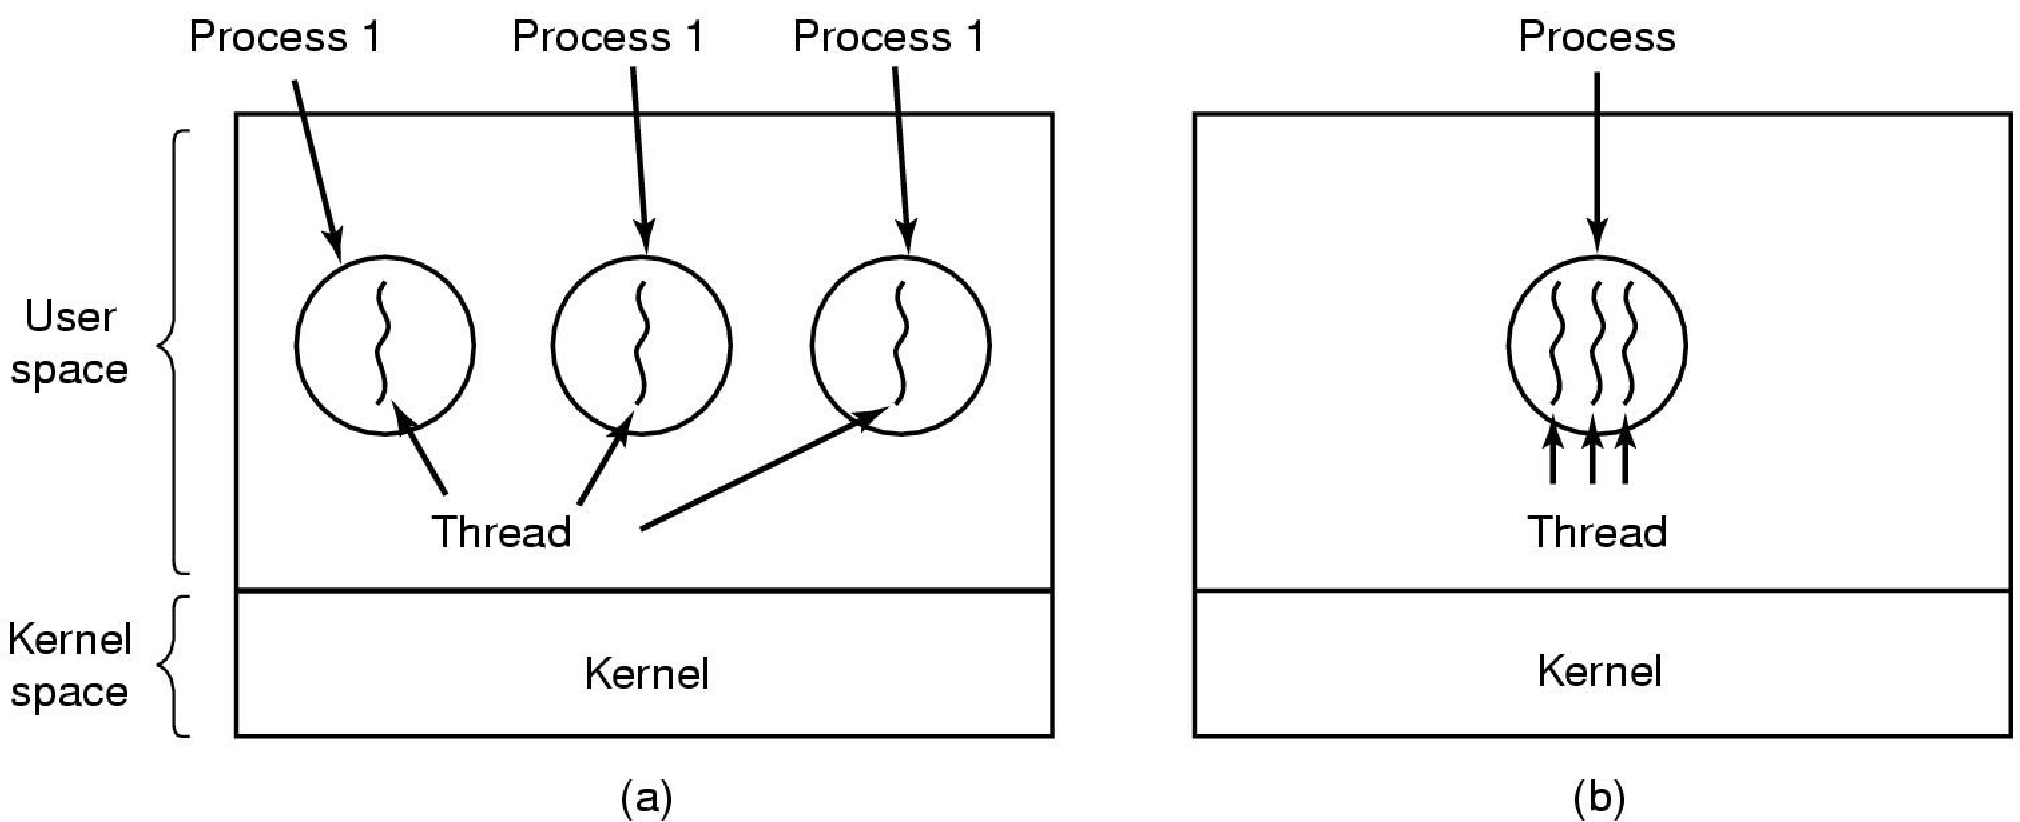
\includegraphics[width=0.7\textwidth]{differences_between_processes_and_threads_1}
	%\caption{Diferencia entre procesos y threads}
	\label{fig:differences_between_processes_and_threads_1}
\end{figure}

\begin{figure}[H]
	\centering
	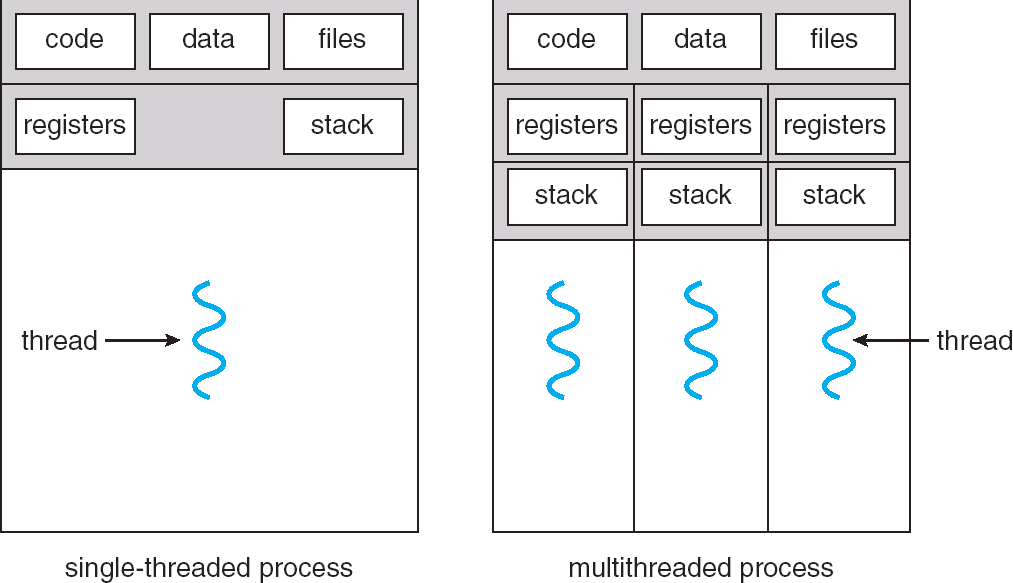
\includegraphics[width=0.7\textwidth]{differences_between_processes_and_threads_2}
	%\caption{Diferencia entre procesos y threads}
	\label{fig:differences_between_processes_and_threads_2}
\end{figure}

\textbf{Thread Control Block (TCB)}

Hay informacion que pasa del PCB al (o los) TCB

\begin{figure}[H]
	\centering
	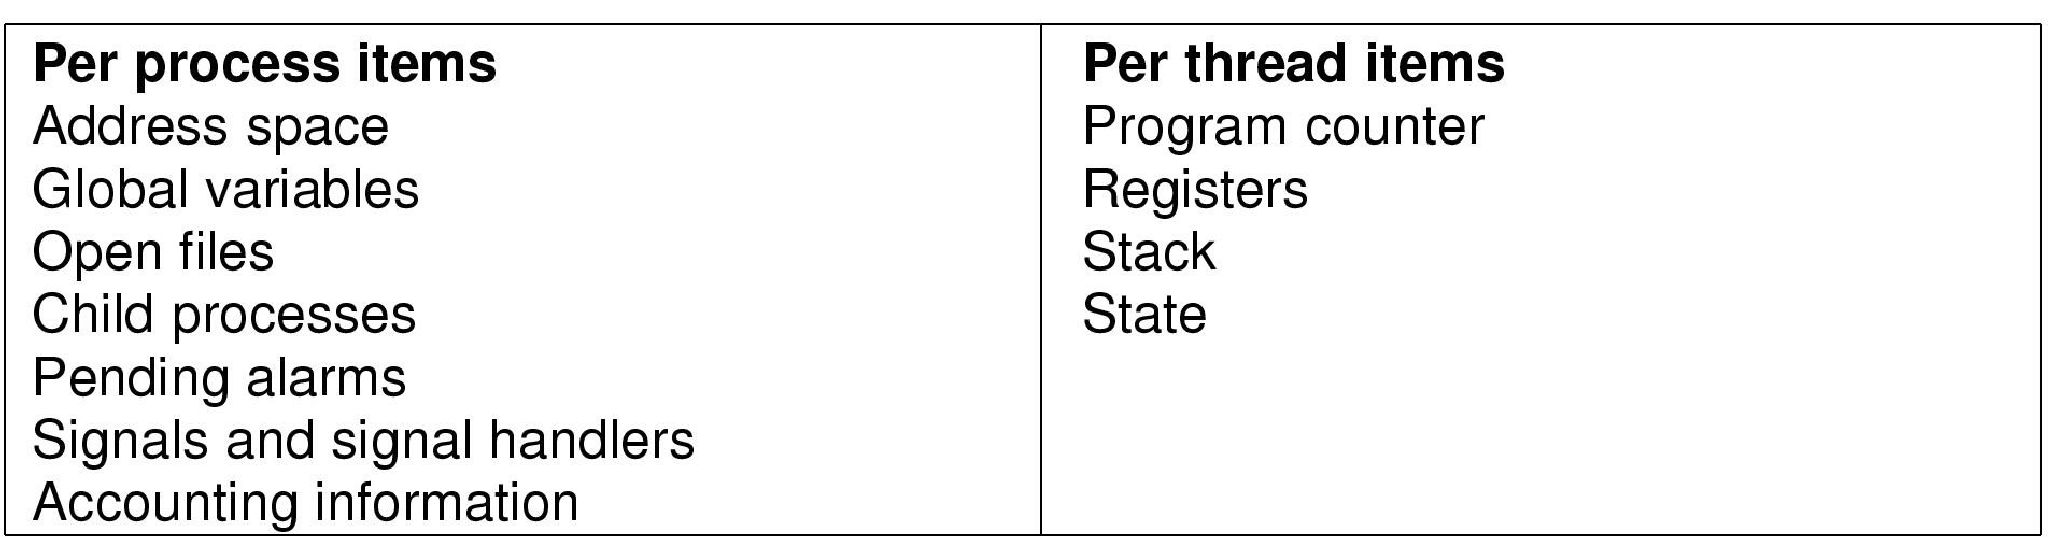
\includegraphics[width=0.7\textwidth]{differences_between_processes_and_threads_3}
	%\caption{Diferencia entre procesos y threads}
	\label{fig:differences_between_processes_and_threads_3}
\end{figure}

Like traditional process, thread can be in any of several states: running, blocked, ready or terminated. A running thread concurrently has the CPU and is active. A blocked thread is waiting for some event (or other thread) to unblock it. A ready thread is scheduled to run and will as soon as its turn come up. The transitions between threads states are the same as transitions between process states.

\subsection{Aplicaciones de multithreading}
Varias aplicaciones que concurren sobre los mismo datos como:
\begin{itemize}
	\item Un server que lanza un thread por cada pedido.
	\item Un procesador de texto concurrente con su corrector y su armador de pagina.
	\item El manejo de Interfaces Gráficas.
\end{itemize}

Algunos de los sistemas hechos con threads podrían hacerse con eventos.

Eventos usan handlers y callbacks, los threads quedan congelados hasta que se les devuelve el control.

Escalar con threads es casi trivial, escalar con eventos tiene un techo (stack ripping) 

No mezclar threads con eventos.

\subsection{Implementacion de threading}
There are two main ways to implement a threads package: in user space and in the kernel (a hybrid implementation is also possible).

\subsubsection{Threads in user space}
The kernel knows nothing about them. As far as the kernel is concerned, it is managing ordinary, single-threaded processes (can be implemented in operating systems than not suport threading). Threads are implemented by a library.

Cada proceso tiene su propia tabla de threads privada, para seguirle el rastro a cada uno de sus threads. En la tabla se guardan las propiedades del thread (program counter, stack pointer, registers, state, etc). La tabla es manejada por el runtime system.

When a thread does something that may cause it to become blocked locally, for example, waiting for another thread in its process to complete some work, it calls a run-time system procedure. This procedure checks to see if the thread must be put in a blocked state. If so, it stores the thread’s registers in the thread table, looks in the table for a ready thread to run, and reloads the machine registers with the new thread’s saved values. As soon as the stack pointer and program counter have been switched, the new thread comes to life again automatically.

La biblioteca de threads permite al usuario multiplexar su time slice.

Time slice: tiempo que puede ejecutarse un proceso sin que el SO lo pare (impide que el usuario bloquee el sistema).\\

\textbf{Ventajas}
\begin{itemize}
	\item Doing thread switching like this is at least an order of magnitude (maybe more) faster than trapping to the kernel. The procedure that saves the thread’s state and the scheduler are just local procedures, so invoking them is much more efficient than making a kernel call. Among other issues, no trap is needed, no context switch is needed, the memory cache need not be flushed, and so on. This makes thread scheduling very fast.
	\item Customized scheduling algorithm.
	\item Scale better, since kernel threads require some table space and stack space in the kernel, which can be a problem if there are a very large number of threads.
\end{itemize}

\textbf{Problemas}
\begin{itemize}
	\item How to implement blocking systems calls. It should prevent one blocked thread from affecting others.
	\item If a thread starts running, no other thread in that process will ever run unless the first thread voluntarily gives up the CPU
\end{itemize}

\begin{figure}[H]
	\centering
	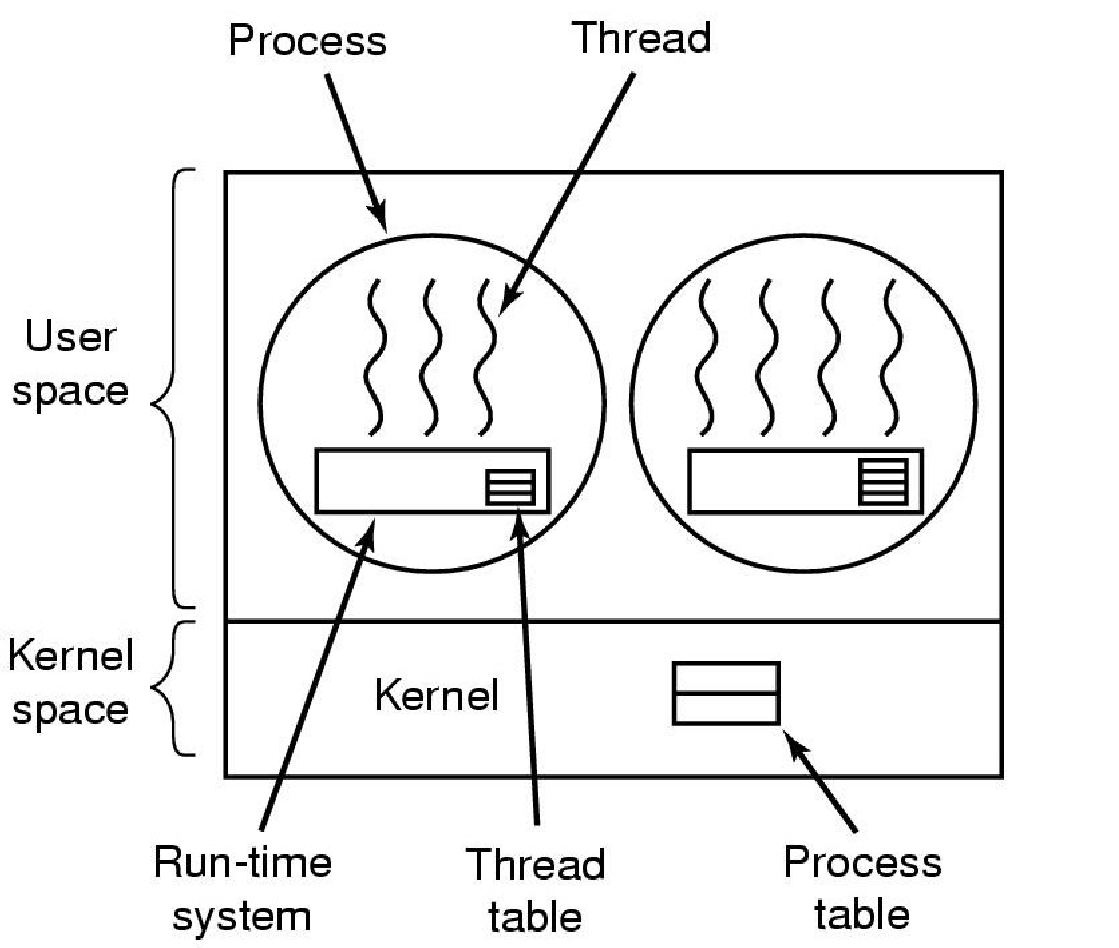
\includegraphics[width=0.7\textwidth]{threads_user_space}
	\caption{Threads en el espacio de usuario}
	\label{fig:threads_user_space}
\end{figure}

\subsubsection{Kernel threads}
The kernel has a thread table that keeps track of all the threads in the system. When a thread wants to create a new thread or destroy an exisiting one, it makes a kernel call, which then does the creation or destruction by updating the kernel thread table.

La tabla del kernel es igual a la que se usa en los threads en el espacio de usuario, pero almacenada en el kernel.

All calls that might block a thread are implemented as system calls, at considerably greater cost than a call to a run-time system procedure. When a thread blocks, the kernel, at its options, can run either another thread from the same process (if one is ready) or a thread from a different process. With user-level threads, the run-time system keeps running threads from its own process until the kernel takes the CPU away from it (or there are no ready threads left to run).

Due to the relatively greater cost of creating and destroying threads in the kernel, some systems recycle their threads. When a thread is destroyed, it is marked as not runnable, but its kernel data structures are not otherwise affected. Later, when a new thread must be ccreated, and old thread is reactivated, saving some overhead.

Kernel threads do not require any new, nonblocking system calls.

Their main disadvantage is that the cost of a system call is substantial, so if thread operations (creation, termination, etc) are common, much more overhead will be incurred.\\

\textbf{Some problems}
\begin{itemize}
	\item Multithreaded process fork: How many threads for the new one?
	\item Signals: when a signal comes in, which thread should handle it?
\end{itemize}

\begin{figure}[H]
	\centering
	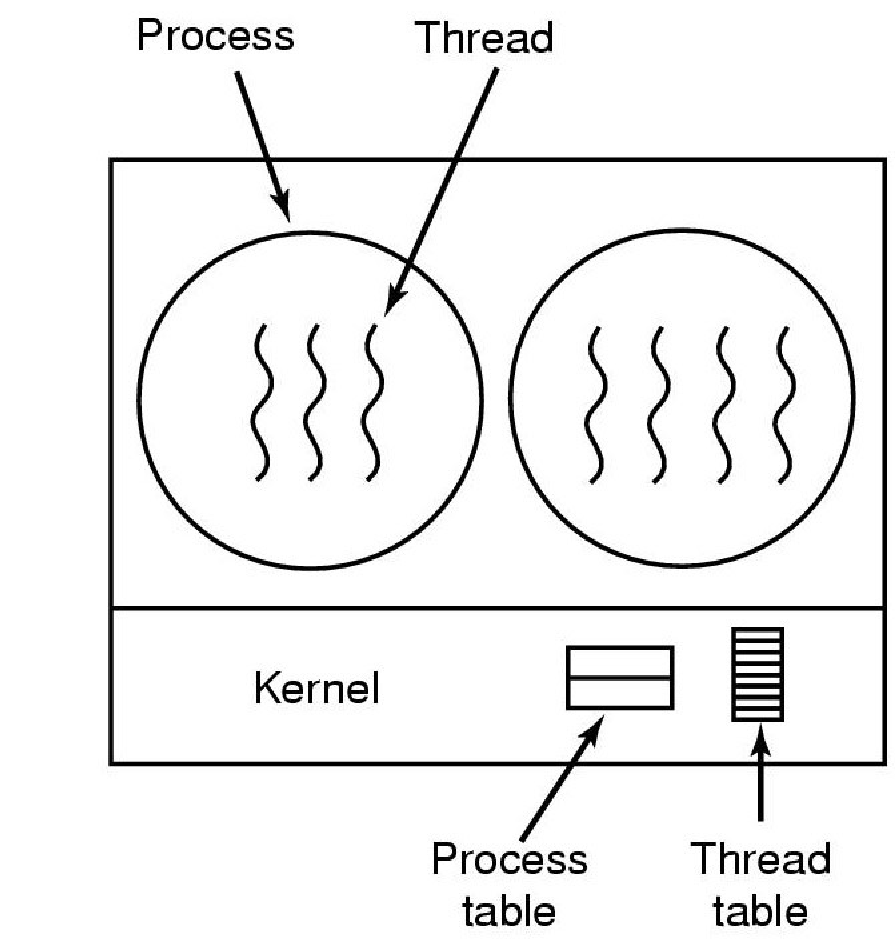
\includegraphics[width=0.7\textwidth]{kernel_threads}
	\caption{Kernel Threads}
	\label{fig:kernel_threads}
\end{figure}

\subsubsection{Implementaciones hibridas}
One way is use kernel-level threads and then multiplex user-level threads onto some or all the kernel threads. The programmer can determine how many kernel threads to use and how many user-level threads to multiplex on each one.

The kernel is aware of only the kernel-level threads and schedules those. Some of those threads may have multiple user-level threads multiplexed on top of them. These user level threads are created, destroyed and scheduled just like user-level threads in a process.Each kernel-level thread has some set of user-level threads that take turns using it.

\begin{figure}[H]
	\centering
	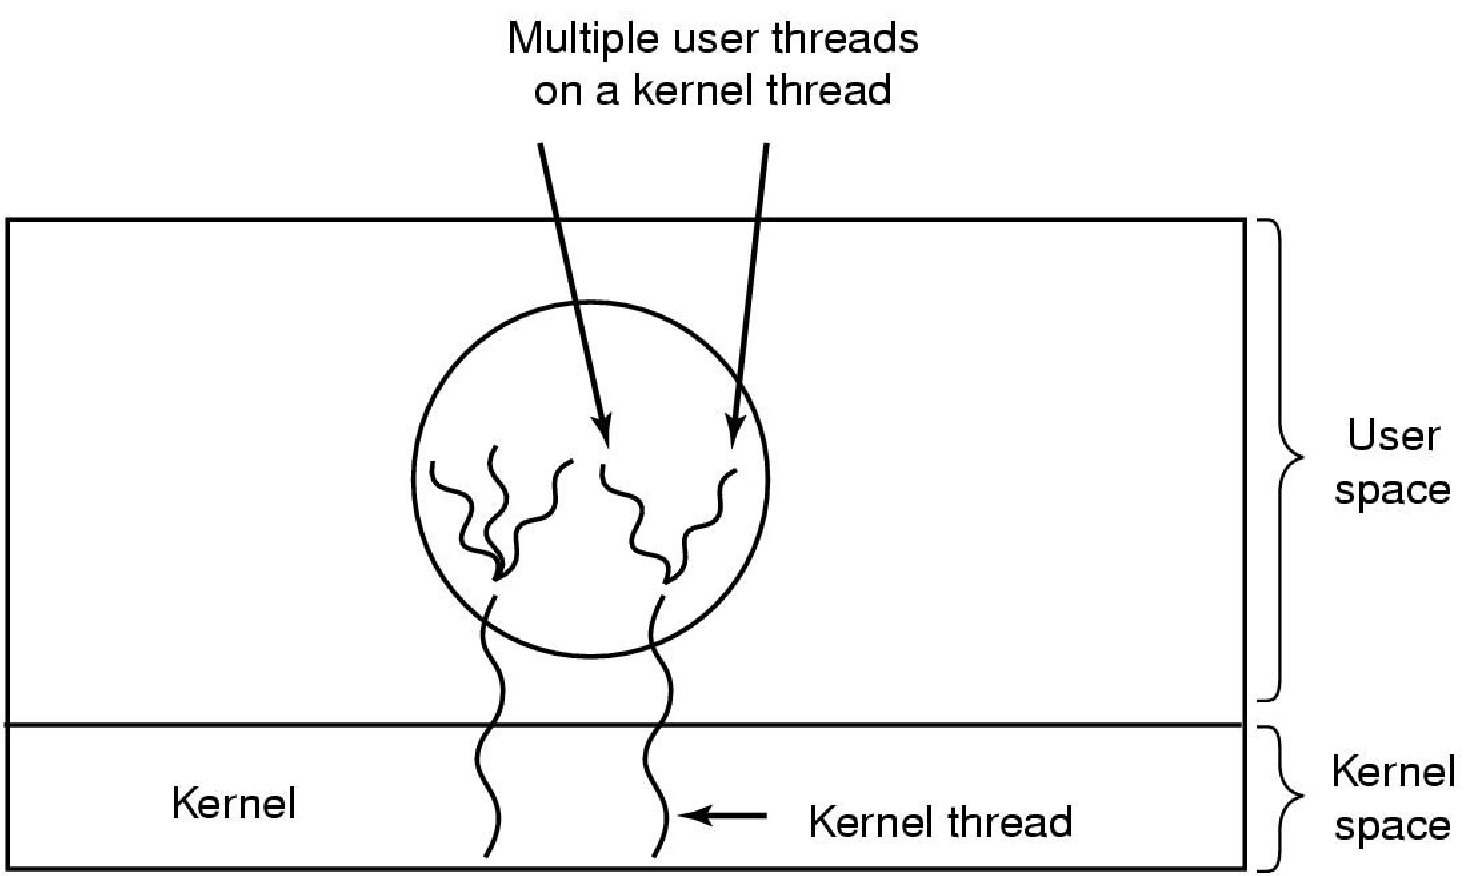
\includegraphics[width=0.7\textwidth]{hybrid_threads}
	\caption{Threads híbridos}
	\label{fig:hybrid_threads}
\end{figure}

\textbf{Scheduler activations}

Mimic the funcionality of kernel threads but with better performance (similar to user space threads).
Cuando se produce una interrupcion, el SO le devuelve el control al usuario.

The kernel assigns a certain number of virtual processors to each process and lets the user space runtime system allocate threads to processors.

The basic idea is that when the kernel knows that a thread has blocked, the kernel notifies the process runtime system by an “upcall”. The runtime system, at its own discretion, can either restart the blocked thread immediately or put it on the ready list to be run later.

An objection to scheduler activations is the fundamental reliance on upcalls, a concept tha violates the structure inherent in any layered system. Normally, layer n offers certain services that layer n+1 can call on, but layer n may not call procedures in layer n + 1. Upcalls do not follow this fundamental principle.

\newpage
\section{Administracion de memoria}

% Bibliografía utilizada en el apunte
\newpage
\newcommand{\bibliographyname}{Bibliografía} % Defino el nombre de la sección de la bibliografía
\addcontentsline{toc}{section}{\bibliographyname} % Agrego la bibliografía en el índice
\renewcommand\refname{\bibliographyname} % Renombro a la bibliografía (por default es 'Referencias')
\begin{thebibliography}{X}
	\bibitem{tanenbaum} \textsc{Andrew S. Tanenbaum}, \textit{Sistemas Operativos Modernos}, tercera edición, PEARSON EDUCACIÓN, México, 2009.
\end{thebibliography}

% Incluir los nombres de las personas que han colaborado en la creación del apunte
%\colaborador{Colaborador 1}
%\colaborador{Colaborador 2}
%\revisor{Dr. Profesor}{10/01/2015}
%\makeseccioncolaboradores % Crea la seccion de colaboradres

% Incluir el historial de cambios
\revision{21/02/2015}{Versión inicial con las secciones de Introduccion, Mecanismos básicos.}
\revision{22/02/2015}{Se agregó la sección de procesos y de threads.}
\makehistorial

\end{document}